% xelatex paper && bibtex paper && xelatex paper && xelatex paper
% xelatex paper && xelatex paper

% NIME 2020 Music Proceedings Template

% Modified December 2019 by Joe Wright
% Created August 2019 by Niccolo Granieri

\documentclass{nimemusic}

\usepackage{lipsum} %used to generate default text
\setcopyright{cc4}
\nimeYear{2024}
\nimeMonth{9}
\nimeDOI{10.1145/XXXXXXX.XXXXXXX}
\whichNIME{NIME’24, 4--6 September, 2024, Utrecht, The Netherlands}

\begin{document}

\newcommand{\CuHum}{\textit{Humming Cumulus}}
\title{Humming Cumulus}

\author{Anonymous Authors}
\affiliation{%
  \institution{Affilitation \#1}
  \city{City}
  \country{Country}
}

\renewcommand{\shortauthors}{Authors, et al.}

\keywords{musical installation, clouds}

\maketitle


\section{Program Notes}

\section{Project Description}
\subsection{Overview}
\CuHum{} is a musical installation/instrument that resembles floating clouds in appearance. The clouds act as the instrument's keys that produce sound, light, and motion when touched.

\begin{figure}[h!]
  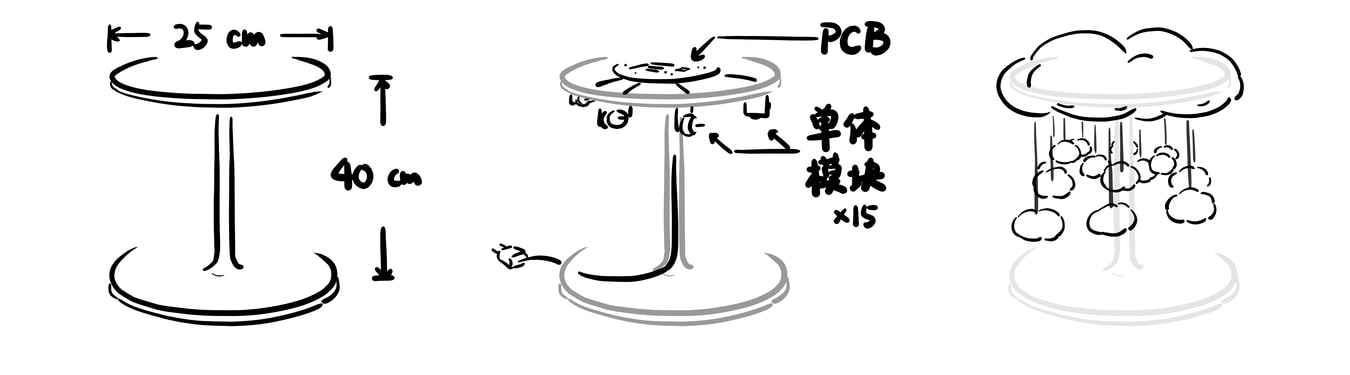
\includegraphics[width=0.95\textwidth]{../../images/CuHum_Appearance.jpg}
  \caption{Sketches of the appearance and composition of the installation.}
  \label{fig:Sketches}
\end{figure}

A guided-play option, selected by holding a special cloud, allows the participant to have clouds fall into their hands in a pre-programmed sequence and play out a tune, creating a tactile and interactive musical experience.

This dual interaction scheme adapts to player expertise, creating opportunities for learning and expression for participants from varied backgrounds. Through our work, we hope to promote musical exploration and social play through an inviting appearance, an easy-to-understand mapping, and rich feedback.

\subsection{Background}
It has been a lasting endeavour for us to bring the joy of musical expression and performance within the reach of those without the advantage of comprehensive musical training and performances -- indeed, music, sounds, and touch are an innate expressive language shared by humankind.

However, musical ``laypeople'' tend to overcomplicate the practice of musical expression and appreciation. We have been constantly witnessing this from friends around us as well as people online: they hold back their intuitive thoughts and comments on sounds; they claim that they ``only listen for sensation's sake'' (with a negative implication) when they go to concerts; they determine that expression and creation is out of their reach because they are ignorant of musical theories; they keep reckoning their inability because they do not score well in rhythm games.

Meanwhile, we see passion surging beneath the surface. We find it a pity that many are gatekept out of this wonderful terrain that they innately connect with. We want to clear up the myth of music's meritocracy as an art form, and invite many more to the play.

Ceaseless sounds from a toy tuned-pipe metallophone in a children's corner struck us awake: what about a toy, an outlet for sound-making as well as an inlet for learning, that guides the player to connect with the music they touch? We put ourselves into the shoes of grown-up children and crafted what we believe we would enjoy --- singing, blinking, playful clouds. We hope they will find resonances around the world, so we bring them to the lovely people at NIME.

On a side note, we also hope they will remotely resonate with the machinery at Utrecht's Museum Speelklok. Who says self-playing bells must be hard metal clockwork? The clouds can find friends anywhere.

\subsection{Design}
\CuHum{} takes the form of a group of small clouds hanging down from a larger cloud above, which is held by a central pillar that supports the weight of other components. The clouds are made of down cotton reinforced with glue and each enfolds a tri-colour LED that gives off breathing lights. Plank makes up the the pillar as well as the casing of the electronic components hidden in the large cloud. Figure~\ref{fig:Sketches} provides a sketch of the overall appearance.

All interaction happens through the participant's hands or arms approaching and touching the clouds. Most of the time, touching one of the cloud triggers a response of the sound of a musical note, the visuals of a changing light, and the haptics of the cloud's bouncing motion. This resembles a conventional instrument-playing experience.

The musical notes follow the diatonic major scale, spanning a register of two octaves, arranged along a circular path. A revolution corresponds to an octave such that notes with the same solf\`{e}ge (full octaves apart) are aligned.

\begin{figure}[h!]
  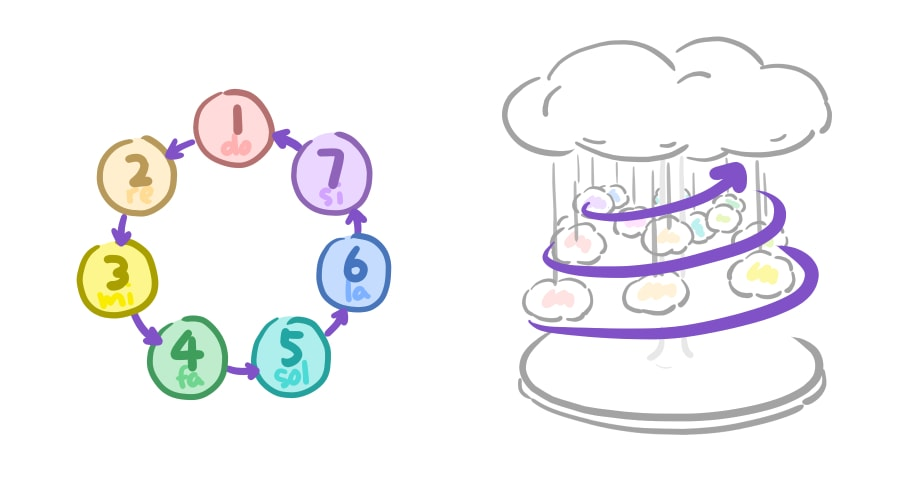
\includegraphics[width=0.75\textwidth]{../../images/CuHum_Solfege.jpg}
  \caption{The solf\`{e}ges and the alignment of the clouds.}
  \label{fig:Solfege}
\end{figure}

A specialty of \CuHum{} is its ``guided play'' mode, which is entered by the participant holding a special cloud marked by a distinctively coloured light. In this mode, clouds descend according to a pre-programmed sequence, and the participant is expected to stretch their hands or arms below all the clouds so that they fall down onto the participant's body.

In this way, we aim to realise the foremost of our intentions --- to expand the reach of the enjoyment of musical engagement. Untrained participants who pass by can try their hands on the instrument as well as go through a tangible, interactive, and understandable journey of the guided play, picking up abundant opportunities for musical exploration and learning. Of course, we expect experienced music practitioners to be getting creative with this new interface, adding to the repertoire of public performances or production techniques, or even tailoring the sounds and hardware to their imagination. We hope that \CuHum{} will be welcoming and inspiring to many.

\subsection{Implementation}
The installation can be built at variable sizes (from tabletop to human-scale) and adapts to different spaces --- we hence omit specific dimensions and give the feasible ranges in Section~\ref{sect:Perf_Notes}. A full prototype is under construction as we have cleared technical difficulties through a series of smaller unit assemblies. In this section, we provide a detailed description of the noteworthy aspects.

\subsubsection{Physical configuration}
At the top of the installation is a circuit board, contained in a plank casing hidden in a large blob of cotton cloud. Power is supplied into the device through the central pillar. Clouds hang down from openings on the bottom of the casing. The previously-shown Figure~\ref{fig:Sketches} displays this overall configuration.

Each cloud is driven by a brushless DC (BLDC) motor also hidden in the large cloud. A spindle is attached to the motor and a bundle of wires is wound around it. The wires are connected to the cloud so that it can be elevated and lowered through rotations of the motor.

The clouds each contains a silver-plated sewing thread, wrapped around the cotton, that serves as the electrode of capacitive sensing. This thread is fixed to an extended electrical wire by copper tape and glue. In addition, the LEDs buried in the clouds also call for electrical connections to the on-board circuitry. We hence add electrical wires to the wrapped wire bundle (totalling 5 strands of 32 AWG, strengthened with fishing wire). Figure X provides a depiction of this structure.

\subsubsection{Electronics}
We design and assemble customised printed circuit boards (PCBs) for all the electronics. The entire device comprises a main unit and 16 sub-units. The main unit is responsible for delivering power and control messages to the sub-units, which each takes care of a cloud. Figure~\ref{fig:Block} shows a block diagram of the major components involved.

\begin{figure}[h!]
  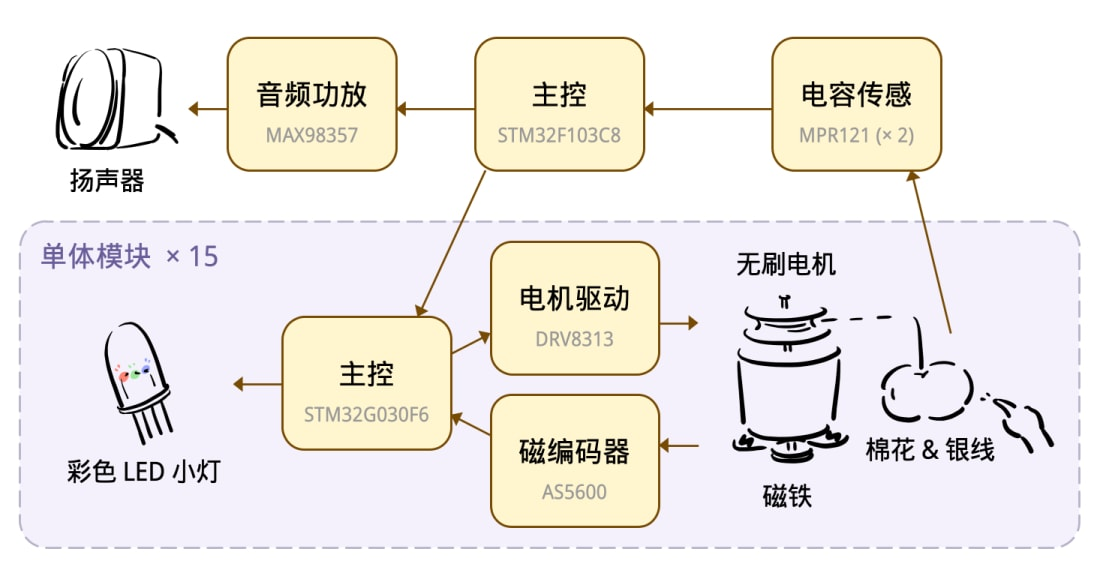
\includegraphics[width=0.9\textwidth]{../../images/CuHum_Block.jpg}
  \caption{Block diagram of electronic components.}
  \label{fig:Block}
\end{figure}

A sub-unit contains a microcontroller communicating with a motor driver and a magnetic encoder which, complemented by the motor equipped with a magnet, forms a vector control closed loop that ensures smooth and silent movements. The main unit monitors readings of the capacitive sensor. When it determines an approaching or a touch has taken place, it sends messages to the sub-units through the SPI protocol indicating desired motor movements and LED lighting patterns. The sub-units continuously runs the motor and the LED on its own, without intervention from the main unit.

We publish all the sources, including mechanical models, circuit board design, and firmware source code, at (anonymised link) under the CC BY-SA licence, in the hope that our implementation details will be useful to interested viewers and future designers.

\subsection{Closing Words}

\section{Performance Notes}
\label{sect:Perf_Notes}

\begin{acks}
Anonymised.
\end{acks}

% \bibliographystyle{nime-music-references.bst}
% \bibliography{nime-references.bib}

\end{document}
\endinput
